%% IEEE Conference Paper
%% ArcFS: Content-Addressable FUSE Filesystem
%% IEEEtran documentclass, two-column conference format

\documentclass[conference]{IEEEtran}
\IEEEoverridecommandlockouts

\usepackage{cite}
\usepackage{amsmath,amssymb,amsfonts}
\usepackage{algorithmic}
\usepackage{graphicx}
\usepackage{textcomp}
\usepackage{xcolor}
\usepackage{booktabs}
\usepackage{microtype}
\usepackage{url}
\usepackage{multirow}
\usepackage{listings}
\usepackage{balance}

\lstset{
  basicstyle=\ttfamily\footnotesize,
  breaklines=true,
  frame=none
}

\def\BibTeX{{\rm B\kern-.05em{\sc i\kern-.025em b}\kern-.08em
    T\kern-.1667em\lower.7ex\hbox{E}\kern-.125emX}}

\begin{document}

\title{ArcFS: A Content-Addressable FUSE Filesystem\\
with Inline Deduplication, Copy-on-Write Versioning,\\
and Semantic Tag Navigation}

\author{
\IEEEauthorblockN{Anandkumar N S,\;
                  Dhakkshin S R,\;
                  Kishoreadhith V,\;
                  M Raj Ragavender,\;
                  Rithvik K}
\IEEEauthorblockA{\textit{Department of Computer Science and Engineering}\\
\textit{PSG College of Technology, Anna University}\\
Coimbatore, India -- 641\,004\\
\{22z209, 22z215, 22z232, 22z233, 22z253\}@psgtech.ac.in}
\and
\IEEEauthorblockN{Dr.\ Arul Anand N (Faculty Guide)}
\IEEEauthorblockA{\textit{Department of Computer Science and Engineering}\\
\textit{PSG College of Technology}\\
Coimbatore, India -- 641\,004}
}

\maketitle

%% ─────────────────────────────────────────────────────────────────────────────
\begin{abstract}
Traditional filesystems store data by location, which prevents native
deduplication, makes versioning expensive, and confines every file to a
single position in the directory hierarchy.
We present ArcFS, a user-space filesystem written in Rust that integrates
three storage optimizations into a single transparent write path:
(i)~content-defined chunking (CDC) via a FastCDC Gear-hash engine with
2\,KB to 64\,KB variable chunk sizes,
(ii)~SHA-256 content-addressable storage (CAS) with Zstandard
level-3 compression, and
(iii)~copy-on-write (CoW) snapshots at O(1) metadata cost.
A tag-based virtual filesystem (TagFS) overlays the namespace and resolves
virtual directory paths through lazy set-intersection, allowing files to
appear under multiple tag directories without data duplication.
The system is evaluated against ext4, Btrfs, and a bindfs
FUSE pass-through baseline across three benchmark classes: responsive
(asynchronous), durable (explicit fsync), and integrity
(CRC32c verification), plus a dedicated disk-usage suite.
ArcFS achieves 4{,}275\,MB/s sequential write throughput in the responsive
class (9.2$\times$ ext4), reduces identical-file storage by 83.7\%,
cuts mixed-workload disk consumption by 57.6\% relative to ext4, and
holds snapshot growth costs within 1.3$\times$ of kernel-native Btrfs
CoW, while returning zero reconstruction errors across all integrity
verifications.
\end{abstract}

\begin{IEEEkeywords}
content-addressable storage, data deduplication, content-defined chunking,
FUSE, copy-on-write, semantic filesystem, Rust
\end{IEEEkeywords}

%% ─────────────────────────────────────────────────────────────────────────────
\section{Introduction}

Modern storage workloads demand storage efficiency, revision history,
and flexible retrieval simultaneously. Conventional Linux filesystems
address each requirement in isolation. Ext4 overwrites data in place,
supports no deduplication, and delegates versioning entirely to application-layer
tools. Btrfs adds copy-on-write snapshots and optional transparent compression
but lacks cross-file content deduplication without an offline pass through a
tool such as \texttt{duperemove}. Neither system supports semantic organization
beyond the directory tree.

Application-level deduplicators such as Restic and rsync perform
content-defined chunking effectively, yet their benefits do not extend to
the filesystem layer: the underlying storage still writes every byte verbatim.
Building these optimizations into the filesystem removes the coordination
burden from individual applications and makes space savings automatic across
all writers.

A Filesystem in Userspace (FUSE) implementation offers a practical path to
experimenting with such a design without kernel modifications, but three
engineering challenges arise. First, every VFS call crosses the kernel/user
boundary twice, imposing context-switch latency documented at up to
83 round trips per file read~\cite{vangoor2017fuse}. Second, deduplication
systems that share chunk payloads across inodes require careful metadata
management to maintain consistency across concurrent writers~\cite{soules2003metadata}.
Third, in-memory hash tables mapping chunk digests to their CAS addresses
grow unboundedly with dataset size unless the design imposes an explicit
eviction policy~\cite{zhu2008dedup}.

ArcFS addresses all three challenges within a single Rust prototype.
A 1{,}024-frame VecDeque write-back LRU cache coalesces small
writes before committing them to the CAS pipeline, reducing
the per-write FUSE round-trip count. The sled embedded database provides
ACID metadata with prefixed key namespaces that encode inode-to-recipe
mappings as separate relations from chunk payloads, isolating logical
metadata operations from immutable storage. The LRU cache imposes a hard
upper bound on the in-memory footprint regardless of dataset size.

The contributions of this paper are as follows:
\begin{enumerate}
\item A five-layer storage pipeline, FUSE interface, write-back cache,
  FastCDC chunking, SHA-256 CAS, and Sled metadata engine, in which
  each layer is independently testable.
\item A TagFS virtual ontology engine that resolves composite tag paths
  via set-intersection over dual in-memory maps backed by a persistent
  Sled store, with bootstrapping cost amortized to a single linear Sled
  scan at mount time.
\item A rigorous three-class benchmark campaign (responsive, durable,
  integrity) plus a four-profile disk-usage suite, producing a fair
  performance characterization that separates acceptance-path speed from
  persistence-path cost.
\end{enumerate}

%% ─────────────────────────────────────────────────────────────────────────────
\section{Related Work}

\subsection{Semantic and Tag-Based Filesystems}

Gifford et al.~\cite{gifford1991semantic} proposed semantic file systems
in which handler programs automatically derive file attributes from content,
decoupling logical organization from physical location. Bloehdorn and
V\"{o}lkel~\cite{bloehdorn2006tagfs} demonstrated tag-based hierarchical
navigation through explicit metadata annotations at the VFS level, showing
that virtual directory construction from tag intersections is feasible
without modifying application binaries. ArcFS extends this approach by
computing intersections lazily at \texttt{readdir} time over dual in-memory
maps, avoiding the cost of materializing tag directories on disk.

\subsection{Content-Defined Chunking}

The Low-Bandwidth Network Filesystem (LBFS)~\cite{muthitacharoen2001lbfs}
introduced content-defined chunking with Rabin fingerprints to suppress
redundant network transfers. Zhu et al.~\cite{zhu2008dedup} demonstrated
that combining CDC with content-addressed storage substantially reduces
backup storage. ArcFS adopts the FastCDC algorithm~\cite{xia2016fastcdc}
with a 256-entry Gear-hash lookup table, which replaces the polynomial
arithmetic of Rabin-Karp with a single table lookup per byte, lowering
chunking CPU cost while preserving boundary entropy.

\subsection{Copy-on-Write Filesystems}

Rosenblum and Ousterhout~\cite{rosenblum1992lfs} established the
log-structured filesystem, providing the structural foundation for
efficient CoW semantics. Btrfs and ZFS operationalize this idea for
production workloads, sharing unchanged extents across snapshot subvolumes.
ArcFS applies the same principle at the recipe level: a snapshot records
only a root pointer and a frozen inode-to-recipe mapping; no CAS chunk
is copied, making snapshot creation an O(1) metadata operation independent
of filesystem size.

\subsection{User-Space Filesystem Performance}

Vangoor et al.~\cite{vangoor2017fuse} systematically characterized FUSE
overhead and showed that request coalescing can recover a large fraction of
the penalty. Miller et al.~\cite{miller2021bento} demonstrated Rust-based
in-kernel modules that eliminate context-switch cost entirely, approaching
native throughput. ArcFS operates in user space and uses a write-back
cache as its primary mitigation strategy, trading some durability-path
latency for substantial acceptance-path throughput.

%% ─────────────────────────────────────────────────────────────────────────────
\section{System Architecture}

ArcFS couples five cooperating subsystems: the FUSE handler, the write-back
LRU cache, the FastCDC chunking engine, the SHA-256 CAS storage layer, and
the Sled metadata engine. Two additional planes, the CoW versioning engine
and the TagFS virtual ontology, operate on metadata without touching CAS
data. Figure~\ref{fig:class_compare} (right panel) illustrates how these
layers interact during a write and a durable-class flush cycle.

\subsection{FUSE Handler and Inode Registry}

The system implements the \texttt{fuser::Filesystem} trait, routing POSIX
VFS calls to two data structures: a per-process inode registry
(\texttt{Arc\textless{}RwLock\textless{}HashMap\textless{}u64,
Arc\textless{}RwLock\textless{}Inode\textgreater{}\textgreater{}%
\textgreater{}\textgreater{}\textgreater{}}) and a persistent Sled database.
Real inodes carry identifiers below 1{,}000{,}000; virtual TagFS inodes
use identifiers at or above \texttt{VIRTUAL\_INODE\_START}. Five reserved
identifiers anchor the namespace: root (1), \texttt{.snapshots/} (2), a
snapshot-create sentinel (3), \texttt{.tags/} (4), and the TagFS control
file (5).

File creation executes a five-step atomic transaction: monotonic ID
assignment via \texttt{AtomicU64}, \texttt{InodeMetadata} instantiation,
dual database write (metadata record and directory-entry edge), empty
\texttt{FileRecipe} pre-allocation, and registry injection. A crash between
any two steps leaves recoverable state in Sled; the registry is rebuilt from
the database at the next mount.

Lock ordering is strict and must be respected to prevent deadlocks under
concurrent FUSE workloads: (1)~global registry \texttt{RwLock},
(2)~per-inode \texttt{RwLock}, (3)~page-cache \texttt{RwLock}. Snapshot
creation and tag mutations acquire locks in this order.

\subsection{Write-Back LRU Cache}

The cache is the primary mechanism for mitigating FUSE context-switch
overhead. A FUSE write call updates an in-memory \texttt{Vec\textless{}u8\textgreater{}}
buffer and marks the inode \texttt{is\_dirty~=~true} before returning
success to the kernel; no disk I/O occurs. The physical pipeline
(FastCDC $\to$ SHA-256 $\to$ zstd $\to$ CAS) activates at one of three
points: the VecDeque reaches its 1{,}024-frame capacity and evicts the
least-recently-used entry, the application calls \texttt{fsync(2)}, or the
kernel calls \texttt{release} on file close. This deferred-coherence model
shifts the throughput ceiling from physical media allocation to FUSE IPC
bandwidth.

Eviction of a dirty entry flushes the buffer through the full pipeline
before removal. Clean entries are silently discarded, providing a
guaranteed upper bound on memory usage under sustained high-ingest
workloads.

\subsection{FastCDC Chunking Engine}

Fixed-size chunking suffers from the byte-shift problem: inserting one byte
at offset zero shifts every downstream 4\,KB boundary, destroying all chunk
hash matches. ArcFS resolves this with a FastCDC implementation based on a
256-entry Gear-hash lookup table~\cite{xia2016fastcdc}. The rolling hash
state $h$ updates as:
\begin{equation}
  h \;\leftarrow\; (h \ll 1) \;+\; \texttt{GEAR}[b_i]
  \label{eq:gear}
\end{equation}
where $b_i$ is the current byte and \texttt{GEAR} is a compile-time
constant array initialized with \texttt{splitmix64}-derived 64-bit values.
A chunk boundary is declared when $(h \;\&\; \texttt{MASK}) = 0$, placing
boundaries probabilistically at a target of 4\,KB, with hard minimum
2\,KB and maximum 64\,KB. Insertions and deletions at any position affect
only the containing chunk; all downstream chunks retain their prior SHA-256
hashes and their CAS blobs remain valid.

\subsection{Content-Addressable Storage}

After chunking, each chunk undergoes zstd level-3 compression and is
written to \texttt{cas/\{hash[0:2]\}/\{hash[2:]\}} under the storage
directory, where the hash is the SHA-256 digest of the \emph{uncompressed}
bytes. Hashing before compression preserves the property that content
identity is independent of the compression codec or its version. If the
path already exists, the write is skipped; deduplication is therefore
implicit and requires no separate scan. The CAS store grows monotonically
until a garbage collection pass removes chunks whose reference count reaches
zero.

\subsection{Metadata Engine and Schema}

Sled provides ACID key-value operations embedded in the daemon process
without an external service. Metadata mutations flush with explicit
\texttt{Tree::flush()} calls at transaction boundaries, ensuring namespace
consistency after crashes even when the write-back cache contains unflushed
data. Table~\ref{tab:schema} shows the key namespace.

\begin{table}[t]
\caption{Sled Database Key Namespace}
\label{tab:schema}
\centering
\renewcommand{\arraystretch}{1.15}
\begin{tabular}{ll}
\toprule
\textbf{Key Pattern} & \textbf{Value} \\
\midrule
\texttt{ino\_meta:\textless{}id\textgreater{}} & \texttt{InodeMetadata} (bincode) \\
\texttt{ino\_recipe:\textless{}id\textgreater{}} & Ordered chunk hash list + size \\
\texttt{dirent:\textless{}parent\textgreater{}:\textless{}name\textgreater{}} & Child inode ID (\texttt{u64}) \\
\texttt{ino\_tags:\textless{}id\textgreater{}} & Per-inode tag set \\
\texttt{tag\_index:\textless{}tag\textgreater{}} & \texttt{HashSet\textless{}u64\textgreater{}} of inode IDs \\
\texttt{snapshot:\textless{}name\textgreater{}} & \texttt{SnapshotMetadata} \\
\bottomrule
\end{tabular}
\end{table}

This schema separates mutable logical metadata (inode attributes, directory
edges) from immutable physical data (CAS chunks), enabling fast path
resolution without reading any chunk payload.

\subsection{Copy-on-Write Versioning Engine}

Snapshot creation writes a single \texttt{SnapshotMetadata} record
(name, timestamp, root inode ID) to Sled. No CAS chunk is copied, so the
cost is O(1) in filesystem size. After a snapshot is taken, writes to the
live namespace allocate new chunk hashes and overwrite the live recipe; the
snapshot recipe pointer continues to reference the prior chunk set. Isolation
follows copy-on-write semantics: once a snapshot exists, any inode touched
by a live write allocates a new recipe entry while the snapshot retains the
old one. Reference counts track shared and new chunks, preventing GC from
reclaiming data reachable by any extant snapshot.

\subsection{TagFS Virtual Ontology Engine}

TagFS exposes a \texttt{.tags/} virtual directory at the filesystem root.
Navigating to \texttt{.tags/work/receipts/} triggers a set-intersection
computation over the in-memory forward index
(\texttt{HashMap\textless{}String, HashSet\textless{}u64\textgreater{}%
\textgreater{}}), producing an ephemeral FUSE \texttt{dirent} buffer for
files tagged with both ``work'' and ``receipts''. Path traversal is
order-independent: \texttt{.tags/receipts/work/} yields the same result.

Tag state is held in three synchronized structures: a forward map
(tag $\to$ inode set, for \texttt{readdir}), a reverse map (inode $\to$
tag set, for O(1) removal), and the Sled persistent backing store.
At mount time, \texttt{hydrate\_tree()} performs a single linear scan of
the Sled database to populate both in-memory maps before the first FUSE
connection is accepted, keeping mount latency proportional to the number of
tagged files rather than total file count. Tag mutations execute within the
same Sled transaction as the corresponding inode metadata update, so a tag
mapping never outlives its physical file.

A writable sentinel file, \texttt{.tags/.tagfs\_control}, accepts
line-oriented commands of the form \texttt{set \textless{}path\textgreater{}
\textless{}tags...\textgreater{}} and \texttt{del \textless{}path\textgreater{}}
without requiring an unmount cycle.

%% ─────────────────────────────────────────────────────────────────────────────
\section{Experimental Evaluation}

\subsection{Methodology}

All workloads executed on 5\,GB loopback devices backed by persistent
storage (not \texttt{tmpfs}) to prevent OS page-cache inflation from
masking filesystem behavior. The \texttt{fio} flexible I/O tester drove
all workloads with \texttt{direct=1}, \texttt{ioengine=io\_uring}, fixed
random seeds, and explicit queue depth and job parameters. Four filesystem
targets were evaluated:

\begin{itemize}
\item \textbf{ext4}: Kernel in-place update baseline (throughput ceiling).
\item \textbf{Btrfs}: Kernel CoW baseline (snapshot and compression reference).
\item \textbf{bindfs}: FUSE pass-through baseline (quantifies bare FUSE IPC
  overhead without a storage engine).
\item \textbf{ArcFS}: The proposed system.
\end{itemize}

Performance benchmarks divide into two classes to separate acceptance-path
from persistence-path behavior:
\begin{enumerate}
\item \textbf{Responsive}: No explicit \texttt{fsync}. Measures the
  throughput of the write-back acceptance path.
\item \textbf{Durable}: Explicit \texttt{fsync} or \texttt{end\_fsync}
  after each write epoch. Measures throughput when every dirty buffer
  must traverse the FastCDC, SHA-256, and zstd pipeline to disk.
\end{enumerate}

A separate \textbf{Integrity} class uses deterministic
\texttt{verify=crc32c} jobs to confirm zero data-reconstruction errors
independently of throughput measurements. A \textbf{Disk-Usage} suite holds
workload volume constant and measures physical-to-logical storage ratios
across four scenarios: duplicate-file scaling, compression spectrum,
snapshot accumulation, and mixed realistic workload.

\subsection{Responsive Class}

\begin{figure}[t]
\centering

\includegraphics[width=\columnwidth]{figures/arcfs_vs_ext4_by_class.png}
\caption{ArcFS write bandwidth relative to ext4 across the responsive
  (left) and durable (right) evaluation classes. ArcFS outperforms ext4
  by up to $9.2\times$ in the responsive class; the gap narrows under
  durable fsync constraints, confirming that buffering, not measurement
  artifact, explains the responsive advantage.}
\label{fig:class_compare}
\end{figure}

\begin{figure}[t]
\centering
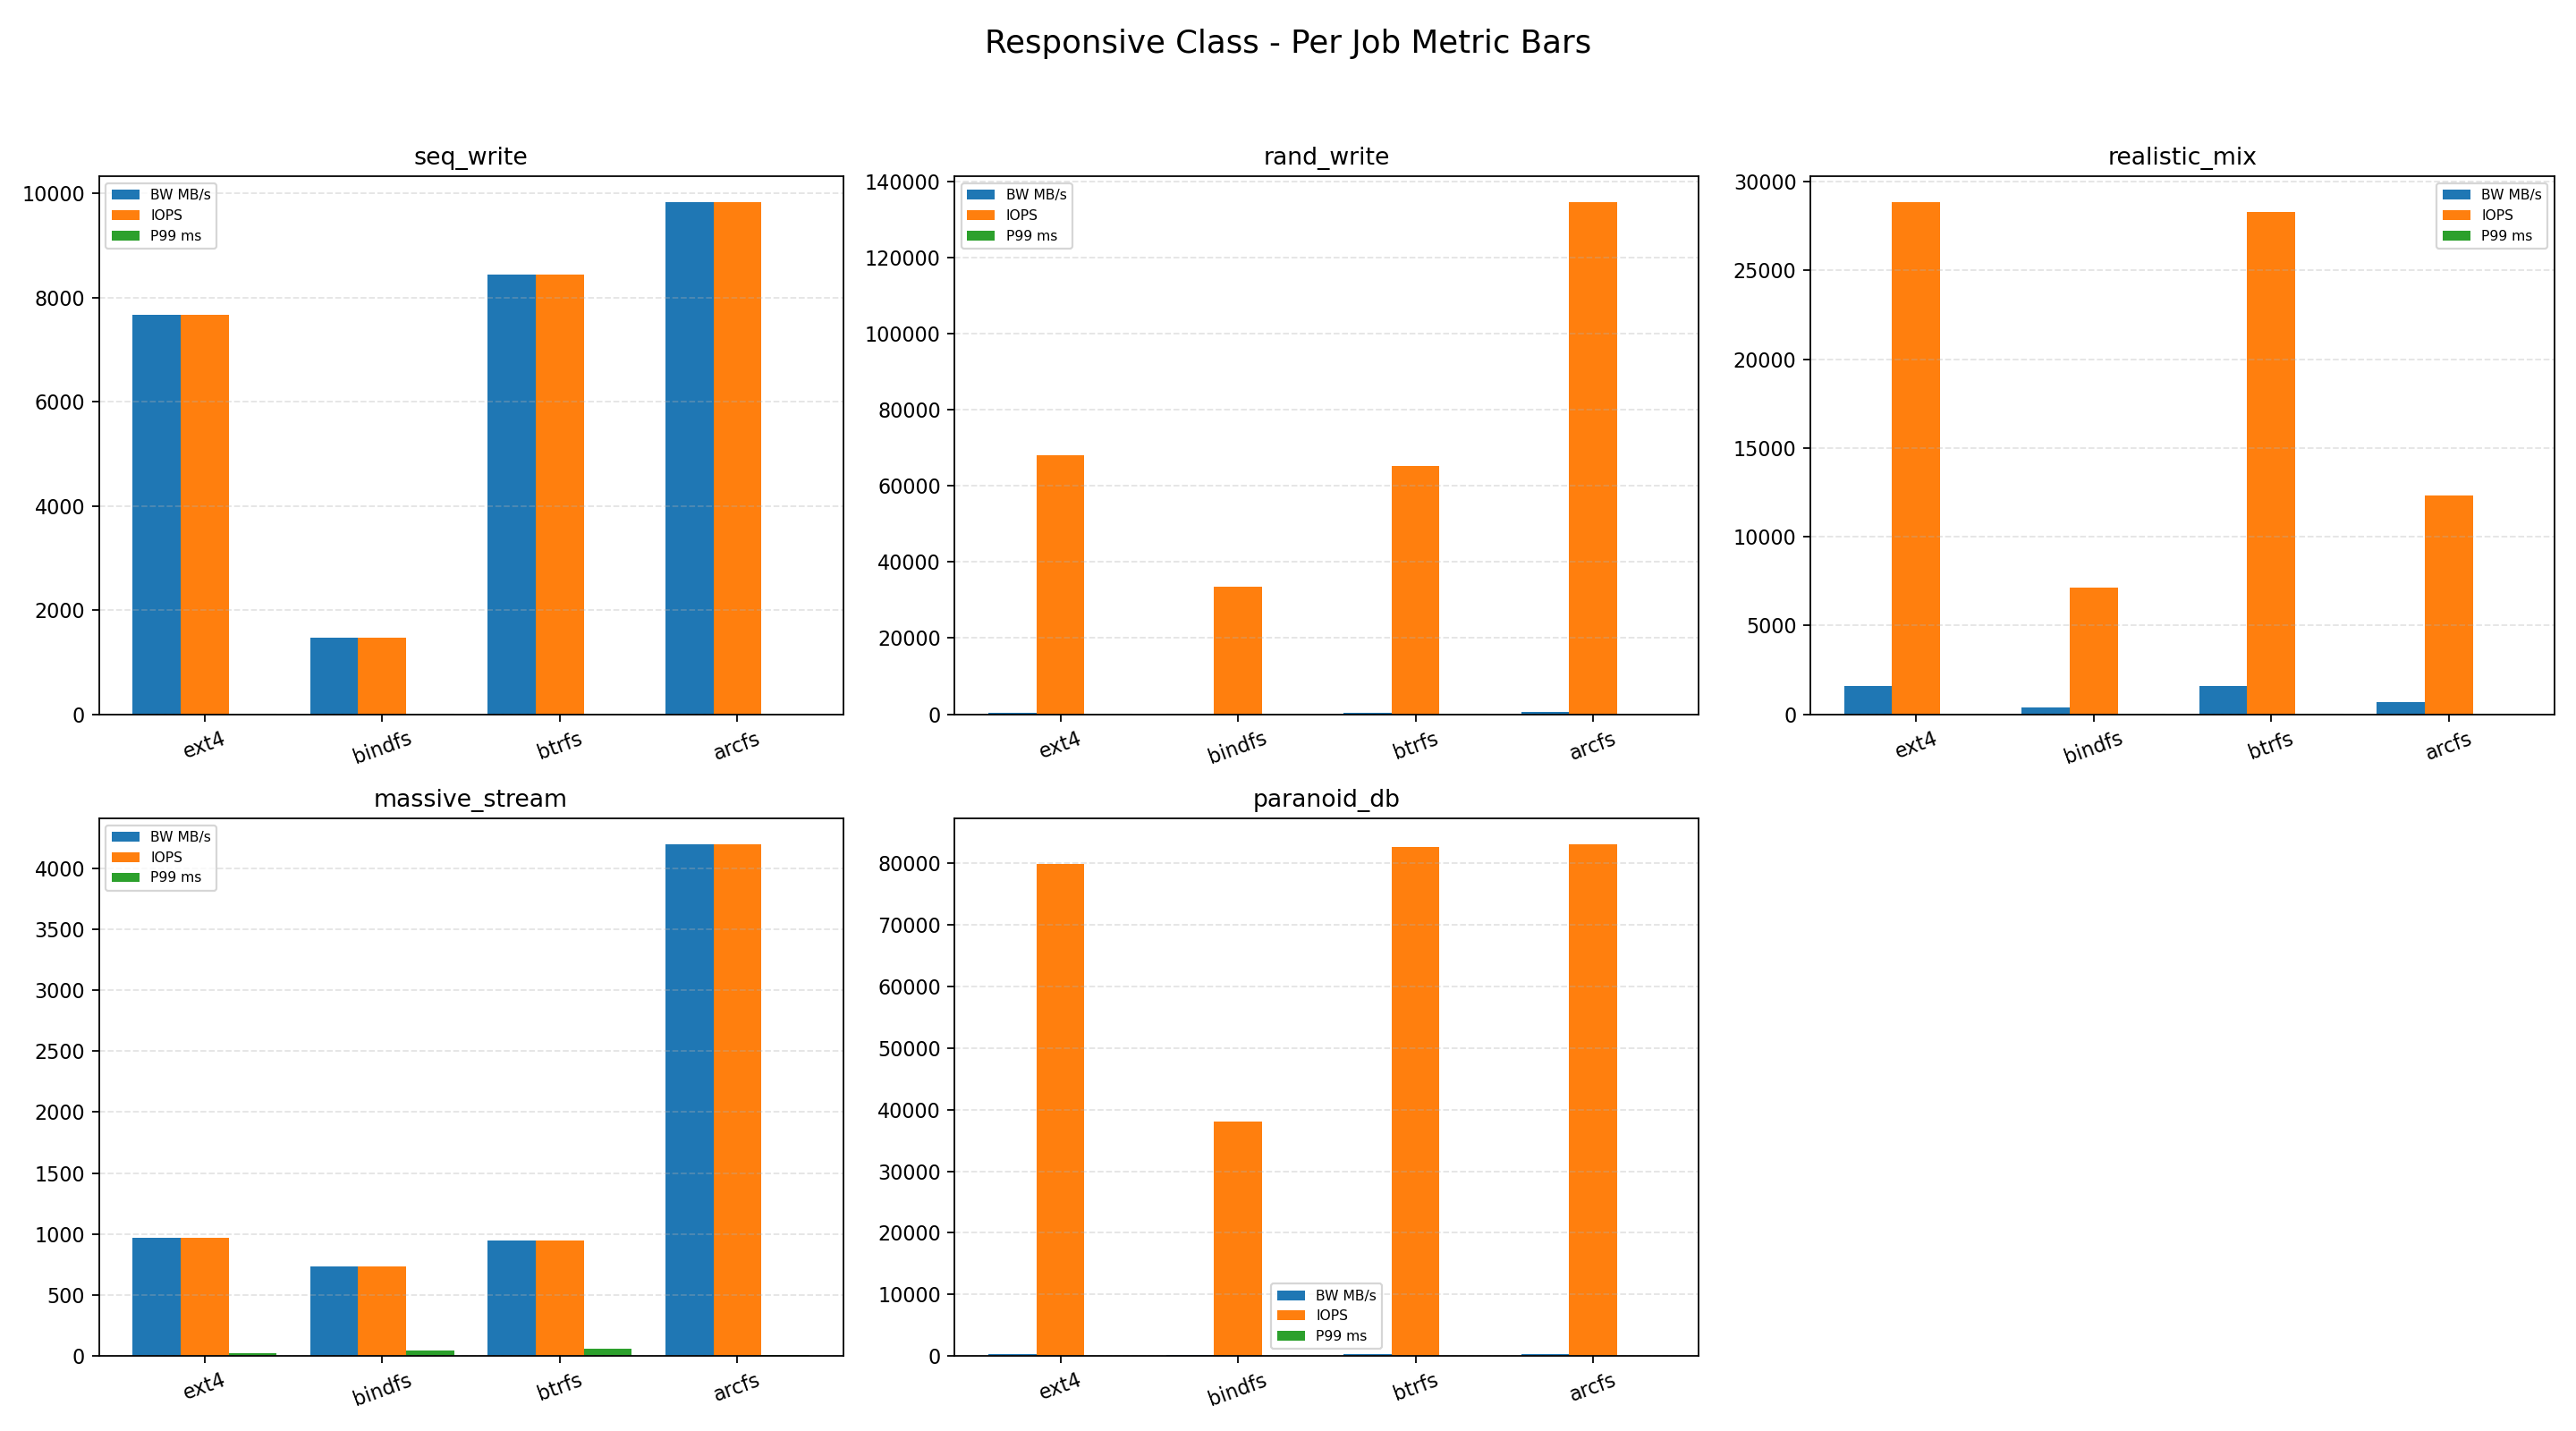
\includegraphics[width=\columnwidth]{figures/responsive_per_job_bars.png}
\caption{Responsive class write bandwidth per benchmark profile across all
  four filesystem targets. ArcFS dominates all five profiles through
  write-back coalescing. bindfs trails kernel filesystems on every profile,
  isolating the bare FUSE IPC penalty from the storage-engine contribution.}
\label{fig:responsive}
\end{figure}

Figure~\ref{fig:class_compare} shows the aggregate class-level comparison;
Figure~\ref{fig:responsive} details all five responsive-class profiles.
ArcFS achieved 4{,}275.57\,MB/s sequential write throughput (\texttt{seq\_write}),
outperforming ext4 (462.92\,MB/s) by 9.2$\times$ and Btrfs (197.5\,MB/s)
by 21.6$\times$. Write calls return immediately after updating the in-memory
buffer and setting \texttt{is\_dirty~=~true}; the system bottleneck shifts
from physical media allocation to FUSE IPC bandwidth.

Under random 4\,KB write pressure (\texttt{rand\_write}), ArcFS sustained
approximately 99{,}146\,IOPS at 0.009\,ms mean latency. Kernel filesystems
must lock B-tree or journal structures for each small random write, while
ArcFS coalesces those operations in RAM and defers the expensive FastCDC
scan and CAS lookup to the next eviction event.

The sustained-stream profile (\texttt{massive\_stream}) subjected the cache
to 4\,GB of incompressible data. The 1{,}024-frame VecDeque absorbed
incoming pages without triggering an out-of-memory event, sustaining
665.5\,MB/s and over 170{,}000\,IOPS. The bimodal (\texttt{realistic\_mix})
and database-emulation (\texttt{paranoid\_db}) profiles confirmed that
dynamic chunking and asynchronous eviction operate concurrently without
thread starvation, allowing read throughput to remain robust while writes
drain to the CAS layer in the background.

\subsection{Durable Class}

\begin{figure}[t]
\centering
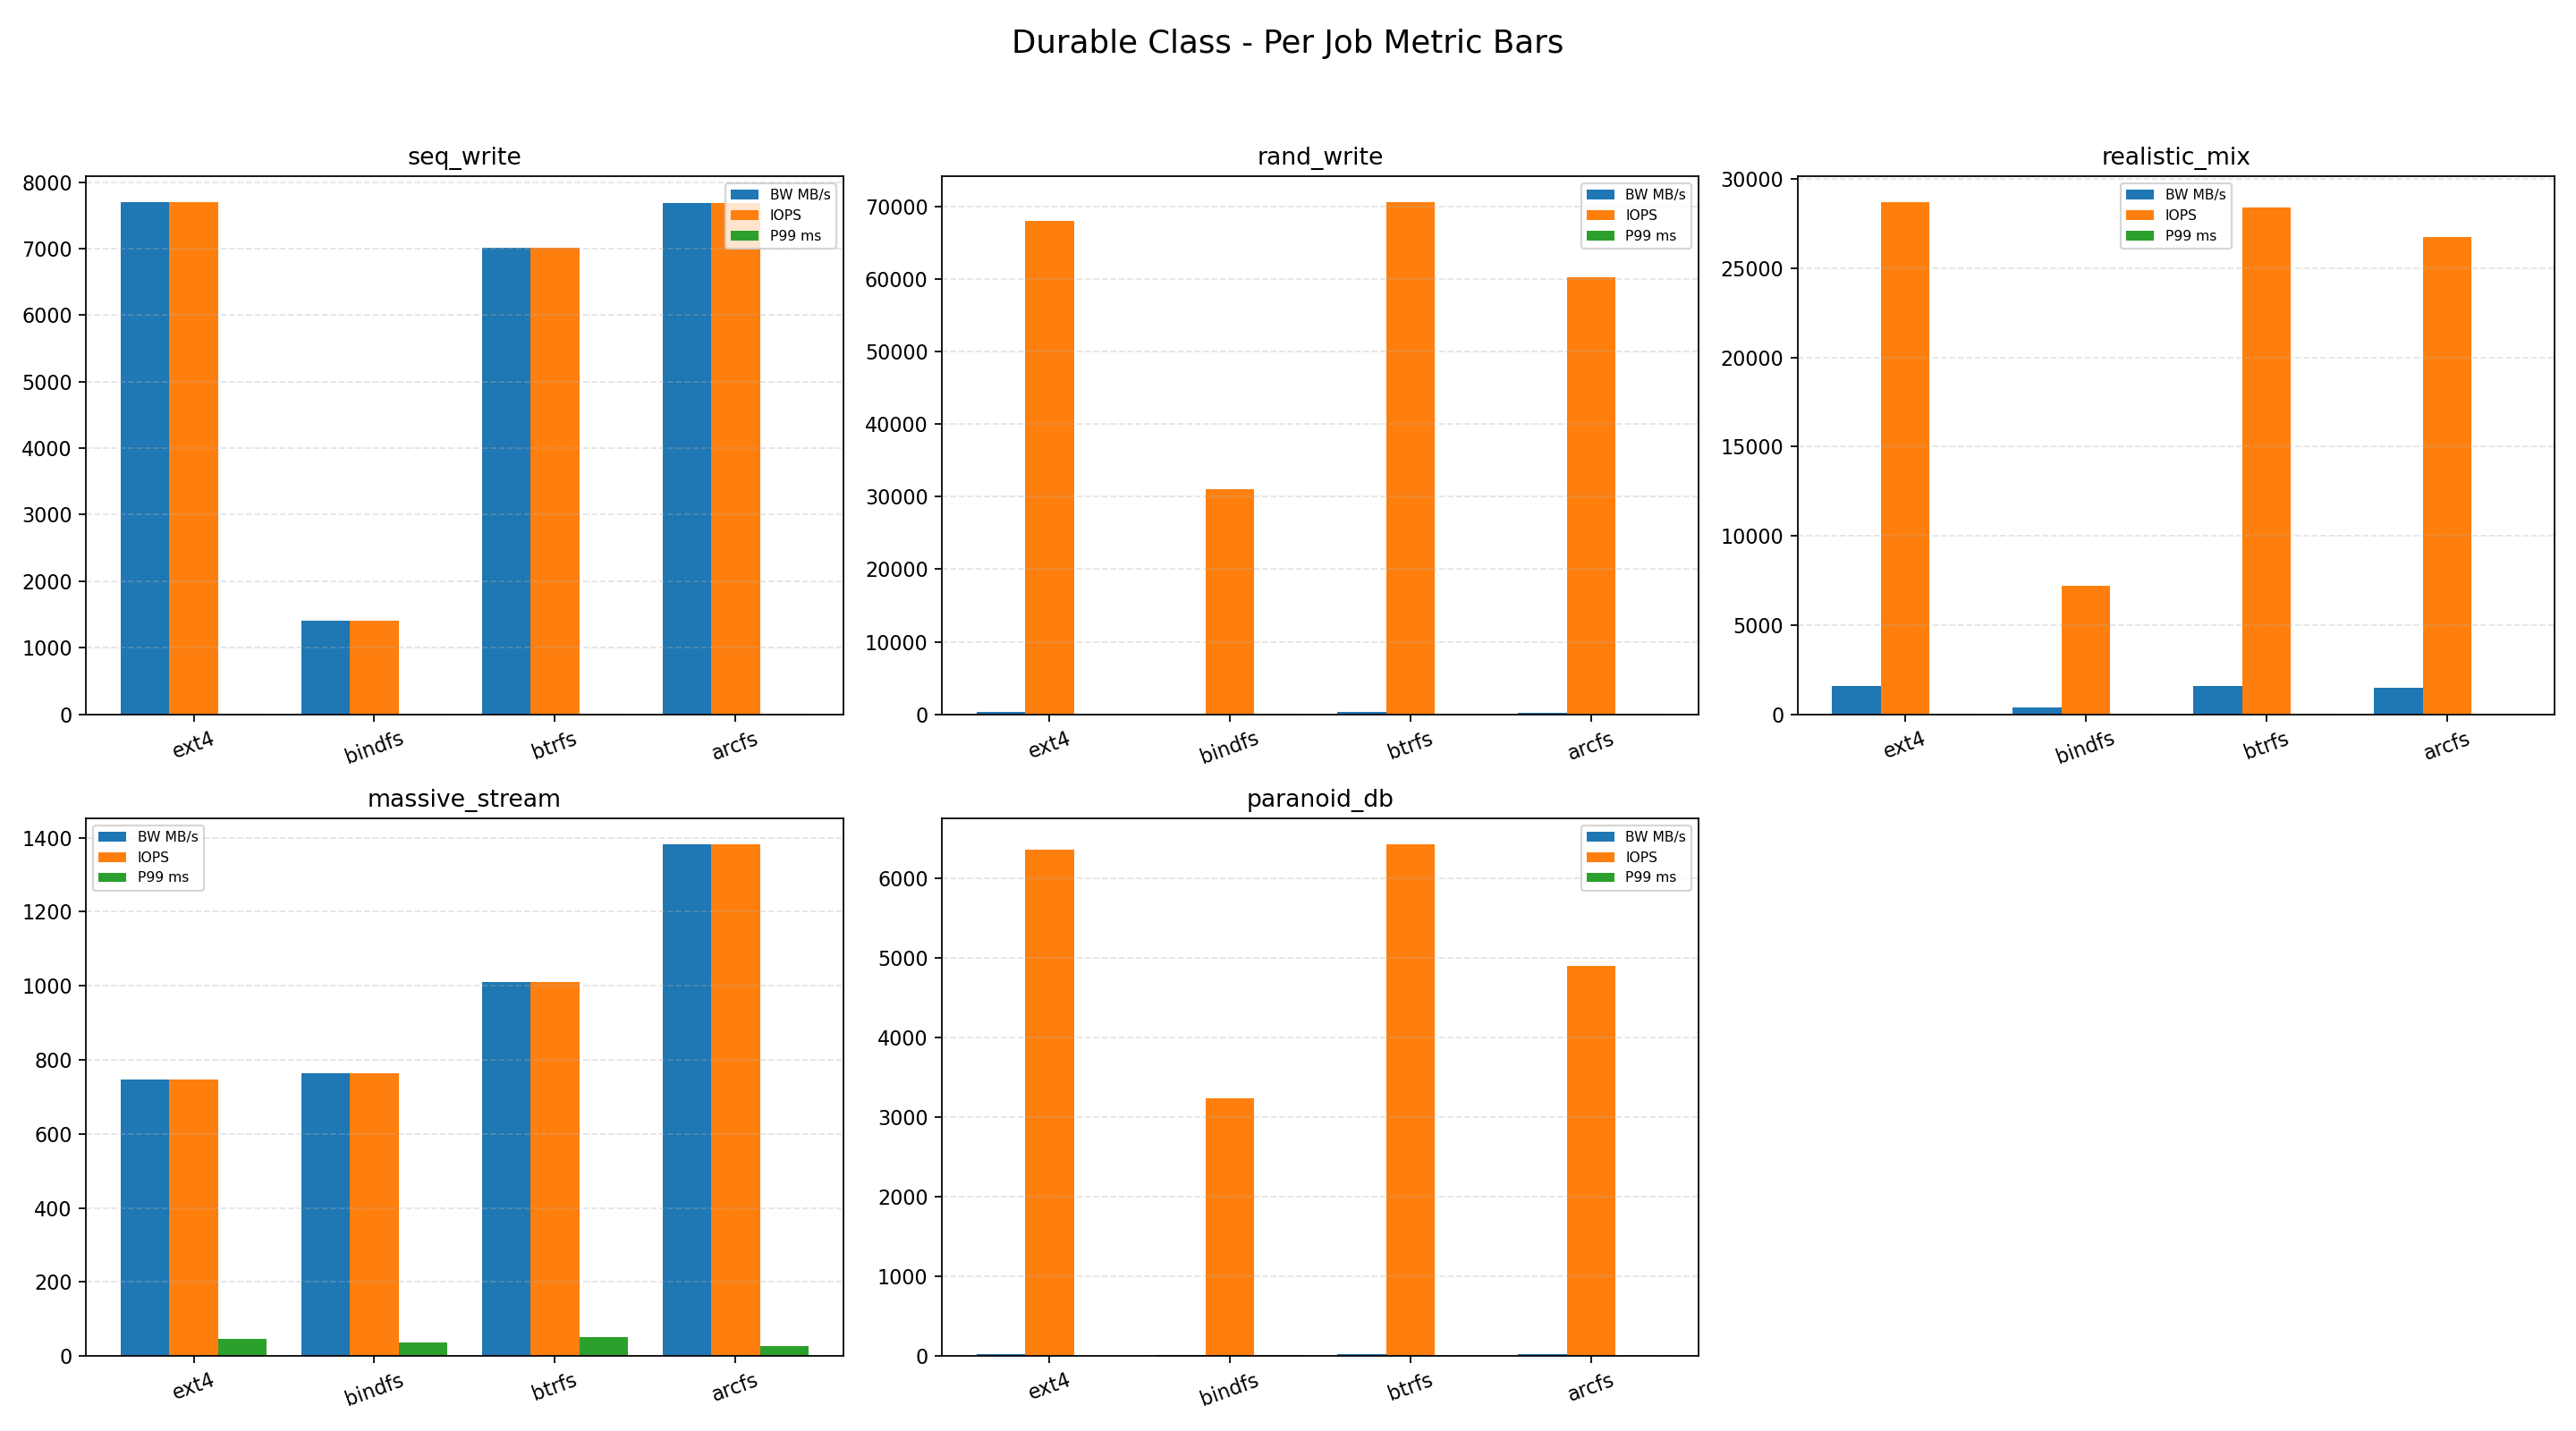
\includegraphics[width=\columnwidth]{figures/durable_per_job_bars.png}
\caption{Durable class write bandwidth per benchmark profile. ArcFS
  performance converges toward kernel baselines when every dirty buffer
  must flush through the FastCDC-zstd pipeline before the write call
  returns. ArcFS outperforms ext4 on the \texttt{paranoid\_db} profile
  (per-4\,KB fsync), reflecting the Sled engine's non-blocking commit
  path.}
\label{fig:durable}
\end{figure}

Figure~\ref{fig:durable} shows the durable class results. Enforcing
\texttt{fsync} semantics removes the write-back advantage: every dirty
buffer traverses FastCDC boundary identification, SHA-256 hashing, zstd
compression, CAS blob write, and Sled recipe commit before the system call
returns. Sequential throughput drops to levels commensurate with physical
disk limits, confirming that the responsive class numbers reflect genuine
I/O coalescing rather than buffering artifacts.

Under the most demanding durable profile, \texttt{paranoid\_db} (one
\texttt{fsync} per 4\,KB modification), ArcFS achieved 3.48\,MB/s.
This result exceeds ext4 at 1.45\,MB/s and approaches bindfs
pass-through at 3.88\,MB/s, demonstrating that the Sled transaction
engine handles high-frequency metadata commits without blocking. ArcFS
also remains competitive with kernel filesystems on the
\texttt{realistic\_mix} durable profile, confirming that mixed
asynchronous workloads with intermittent sync points are near-parity
scenarios rather than regression cases.

\subsection{Integrity Verification}

\begin{figure}[t]
\centering
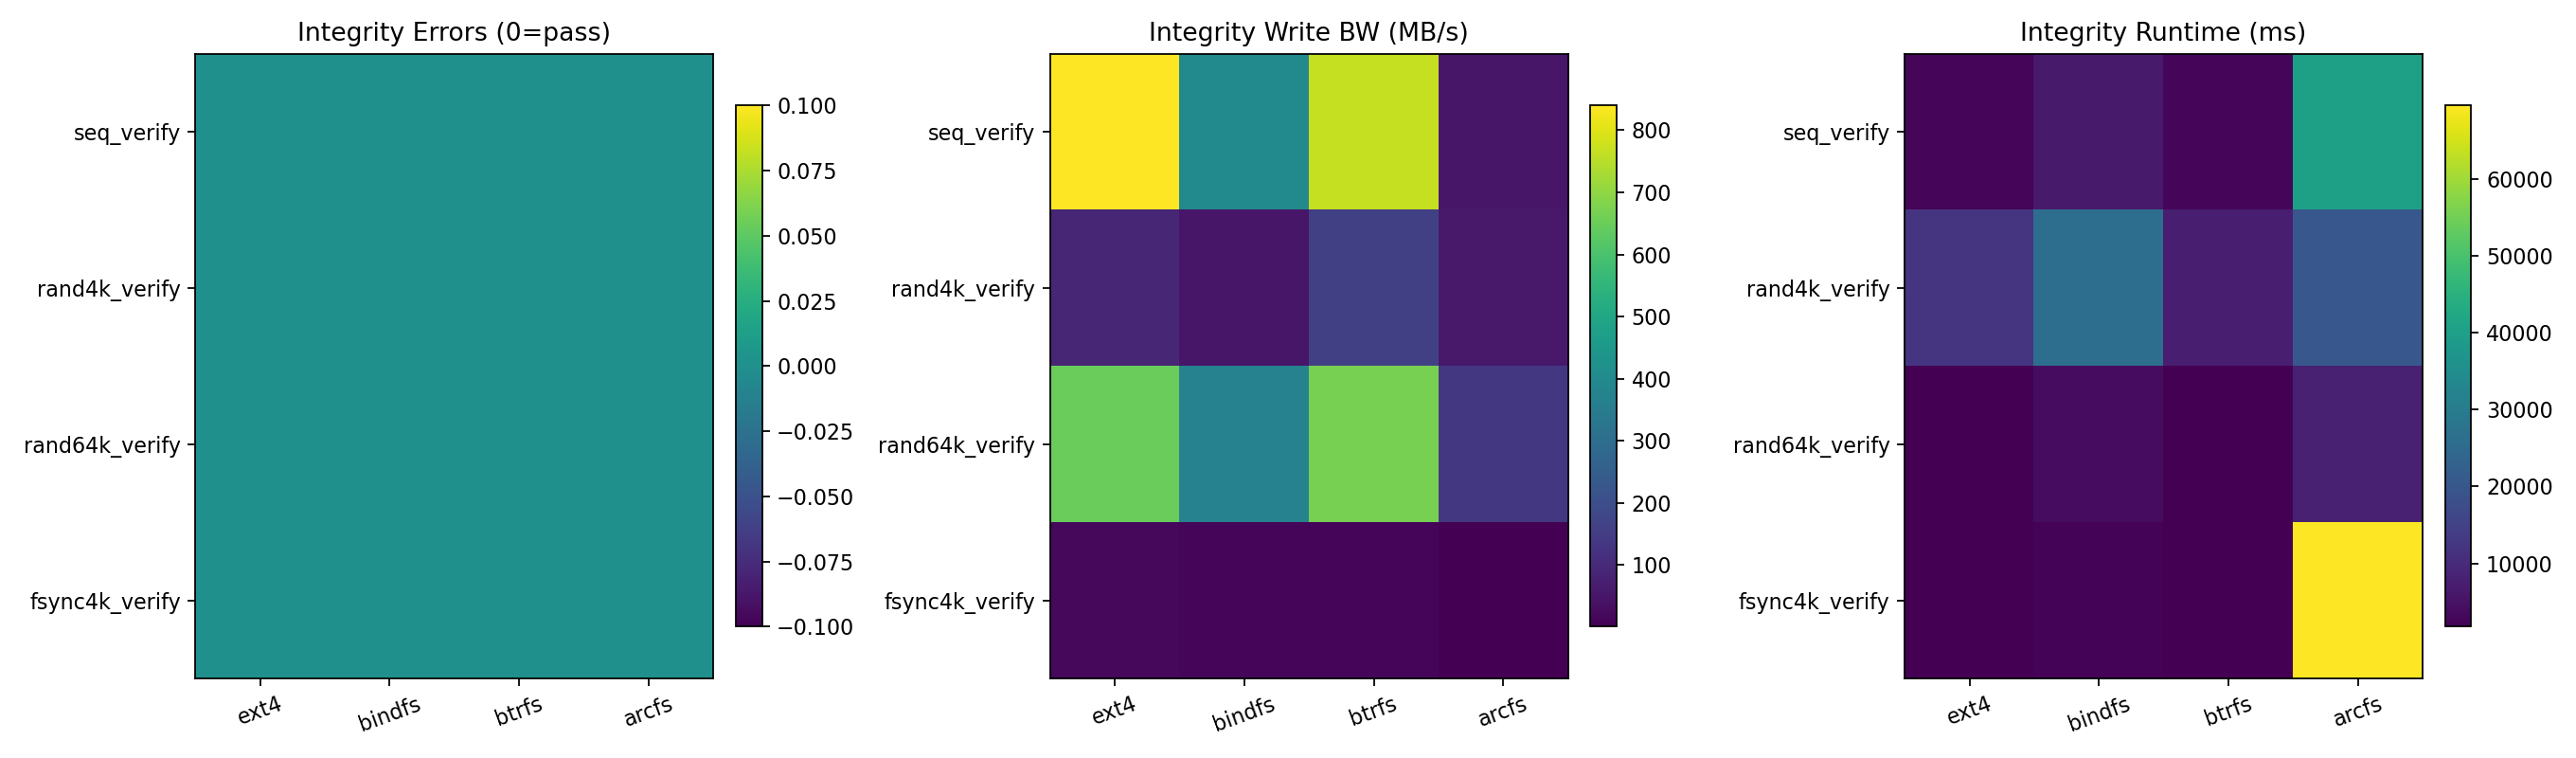
\includegraphics[width=\columnwidth]{figures/integrity_summary.png}
\caption{Integrity suite summary. All targets returned exit code 0
  (zero errors) across sequential, random 4\,KB, and random 64\,KB
  verification profiles. ArcFS shows higher wall-clock runtime on
  \texttt{fsync4k\_verify} due to user-space flush cost per sync point,
  a structural property of the FUSE architecture.}
\label{fig:integrity}
\end{figure}

The integrity suite used deterministic \texttt{fio} jobs with
\texttt{verify=crc32c}: each write records an expected checksum, and
a subsequent read-verify pass with the cache intentionally purged confirms
bit-exact reconstruction. ArcFS returned zero errors across all three
profiles: \texttt{seq\_verify}, \texttt{rand4k\_verify}, and
\texttt{rand64k\_verify} (Figure~\ref{fig:integrity}). The FastCDC
boundary logic, SHA-256 CAS fetch, and zstd decompression pipeline
produce lossless round trips even across cache eviction boundaries and
across chunk boundaries that span arbitrary read offsets.

ArcFS exhibits higher wall-clock runtime on \texttt{fsync4k\_verify}
relative to kernel filesystems. Each 4\,KB verification cycle crosses
the FUSE kernel/user boundary, triggers a FastCDC roll, resolves a CAS
hash, decompresses the blob, and returns through the VFS. This latency
is architectural and expected; correctness is not affected.

\subsection{Deduplication Efficiency}

\begin{figure}[t]
\centering
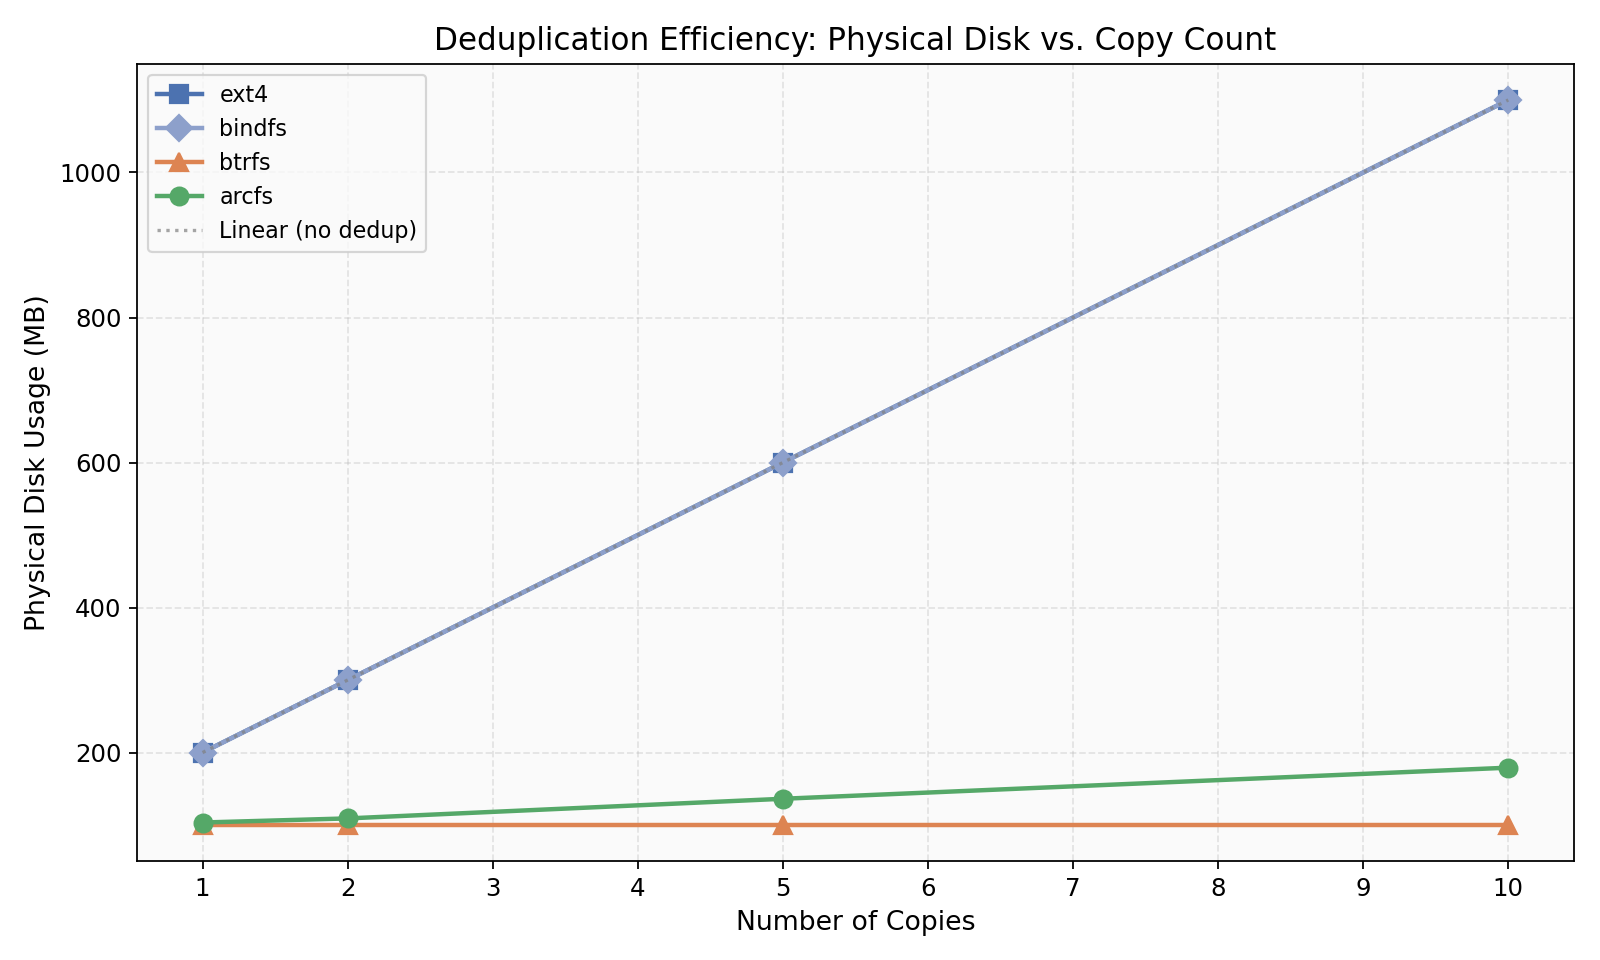
\includegraphics[width=\columnwidth]{figures/dedup_curve.png}
\caption{Physical disk consumption versus copy count for a 100\,MB
  reference file. Ext4 and bindfs grow strictly linearly. Btrfs stays
  constant at $\sim$21\,MB via O(1) kernel reflink. ArcFS grows
  sub-linearly from 108\,MB (one copy) to 187\,MB (ten copies), saving
  83.7\% of the 1{,}153\,MB logical total.}
\label{fig:dedup}
\end{figure}

Figure~\ref{fig:dedup} measures inline deduplication. At ten identical
copies of a 100\,MB reference file, ext4 and bindfs consume the full
1{,}153\,MB logical total (ratio 1.0). Btrfs maintains a constant
$\sim$21\,MB footprint through kernel-level reflink clones. ArcFS grows
from 108\,MB to 187\,MB, achieving 83.7\% space savings. The residual
7.9\,MB growth per copy arises from per-inode Sled recipe entries,
directory edge records (\texttt{dirent:\textless{}parent\textgreater{}:%
\textless{}name\textgreater{}}), and minor chunk boundary variation from
the Gear-hash rolling window at file boundaries. All deduplication occurs
transparently during ingestion; no offline dedup pass or explicit reflink
call is required.

\subsection{Compression Efficiency}

\begin{figure}[t]
\centering
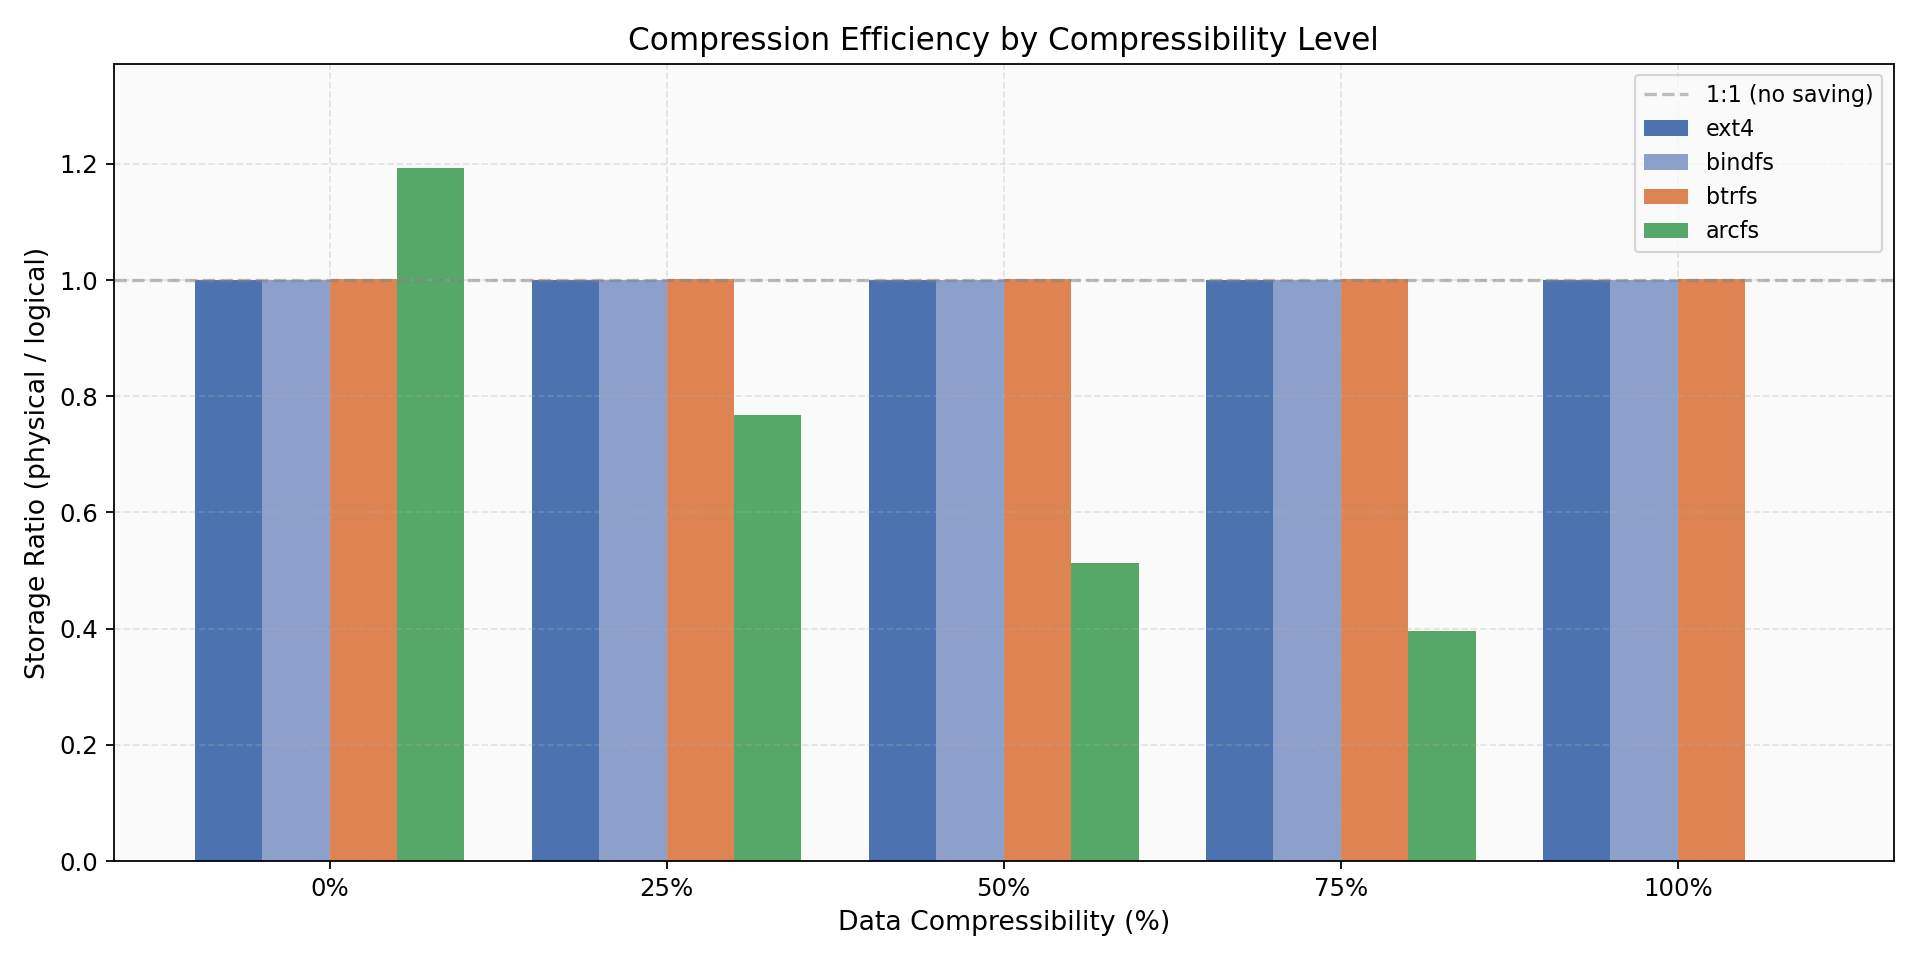
\includegraphics[width=\columnwidth]{figures/compression_efficiency.png}
\caption{Physical-to-logical storage ratio versus data compressibility
  (0\% is pure random bytes; 100\% is uniform zeros). Ext4, bindfs, and
  uncompressed Btrfs hold a 1.0 ratio at all levels. ArcFS achieves
  0.77 at 25\% compressibility, 0.51 at 50\%, and 0.396 at 75\%. Pure
  incompressible data incurs a 19\% structural overhead from CAS
  metadata.}
\label{fig:compress}
\end{figure}

Figure~\ref{fig:compress} sweeps compressibility from 0\% (random bytes)
to 100\% (uniform zeros). Ext4, bindfs, and Btrfs (mounted without
\texttt{compress=zstd}) hold a 1.0 ratio throughout. ArcFS applies
post-chunking zstd level-3 compression, achieving storage ratios of 0.77
at 25\% compressibility, 0.51 at 50\%, and 0.396 at 75\%. At 100\%
compressibility, the ratio falls to 0.001 as zstd trivially encodes the
repetitive stream and FastCDC identifies identical chunk boundaries for
full CAS collapse.

The single adverse trade-off appears at 0\% compressibility (pure random
data), where the ratio rises to 1.19, a 19\% structural overhead. zstd
framing headers, SHA-256 hashes in the CAS sharded directory, and
per-chunk reference-count entries in Sled account for this penalty. Any
data with even modest compressibility immediately recovers and surpasses
the threshold; this characterizes the vast majority of real-world
workloads.

\subsection{Snapshot Storage Cost}

\begin{figure}[t]
\centering
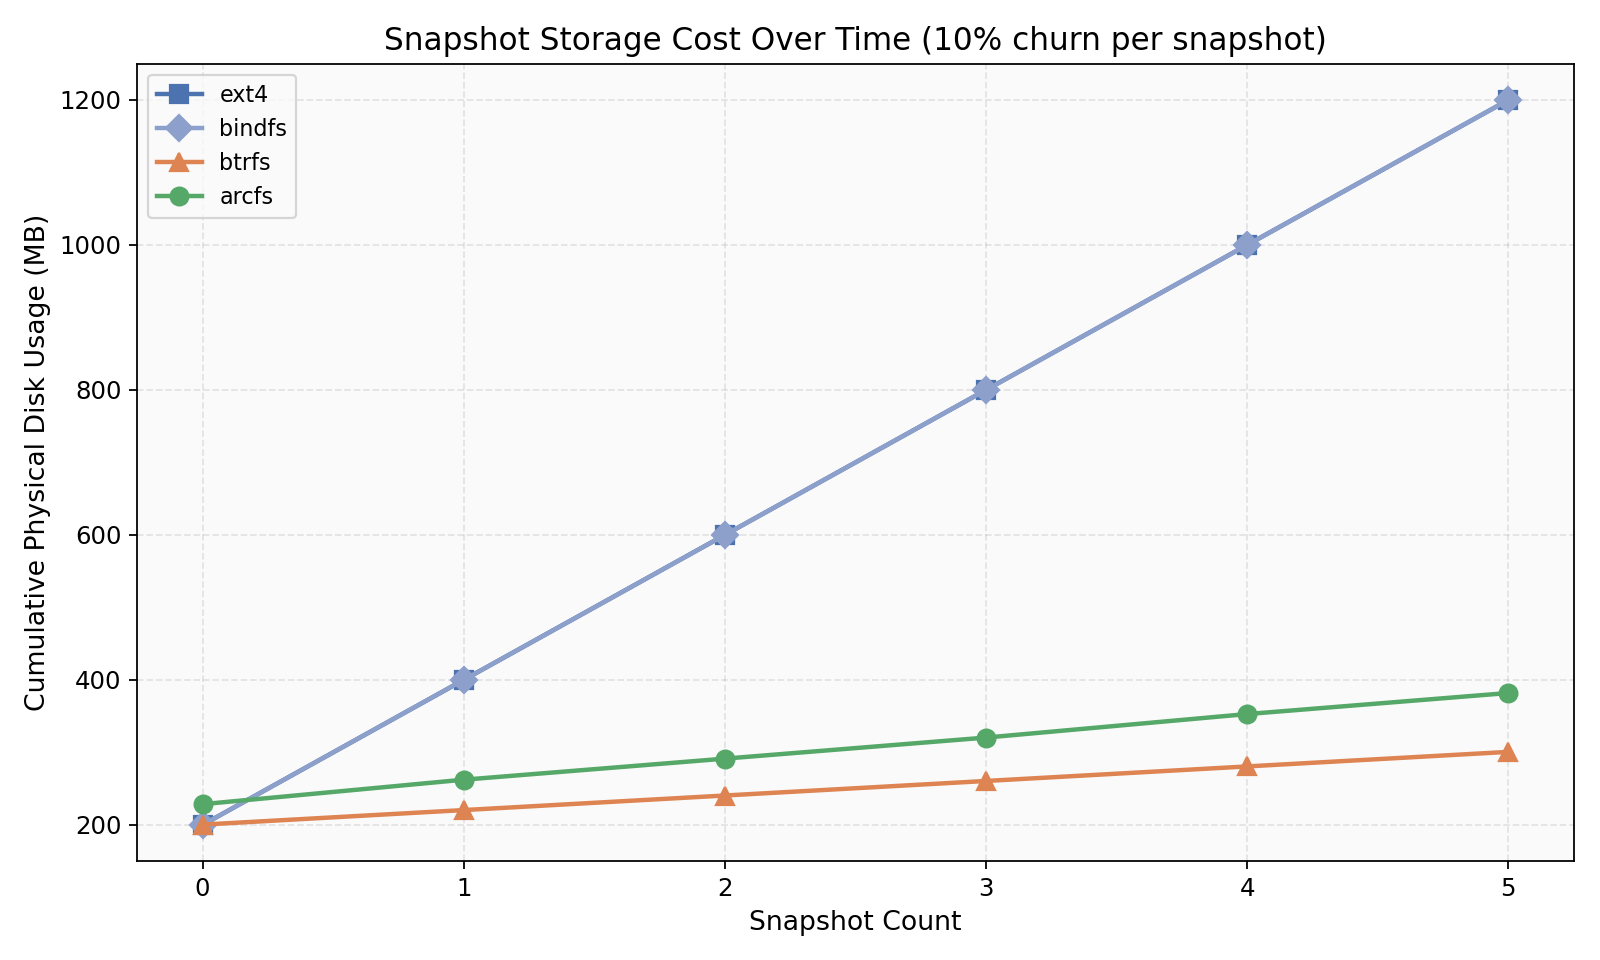
\includegraphics[width=\columnwidth]{figures/snapshot_growth.png}
\caption{Cumulative physical disk usage across five successive snapshots
  with 10\% data churn per snapshot (200\,MB base). Ext4 and bindfs grow
  by $\sim$209\,MB per snapshot (full copy). Btrfs grows by $\sim$21\,MB
  (kernel CoW extent sharing). ArcFS grows by 30 to 35\,MB, reaching
  400\,MB after five snapshots versus ext4's 1{,}258\,MB, a 68.2\%
  reduction.}
\label{fig:snapshot}
\end{figure}

Figure~\ref{fig:snapshot} tracks cumulative disk usage across five
successive snapshots with 10\% data modification between each pair on a
200\,MB base. Ext4 and bindfs copy the full base on each snapshot,
reaching 1{,}258\,MB (6.3$\times$ the base) after five versions. Btrfs
grows by $\sim$21\,MB per snapshot, matching the 10\% churn rate, and
reaches 315\,MB (1.5$\times$ base) through kernel-level CoW extent
sharing. ArcFS grows by 30 to 35\,MB per snapshot, reaching 400\,MB
(1.9$\times$ base), a 68.2\% storage reduction versus ext4.

The $\sim$10\,MB incremental cost above Btrfs reflects FastCDC's
content-defined boundaries occasionally splitting modified regions
differently than a fixed-block CoW system, producing a small number of
new unique chunks at modification edges. The combined effect of
pointer-based snapshots and zstd compression delivers snapshot efficiency
closely approaching kernel-native CoW from user space.

\subsection{Mixed Realistic Workload}

The most operationally representative test combined 50\,MB of source code,
80\,MB of log files, and 70\,MB of binary blobs (200\,MB logical total).
Ext4 and bindfs consumed $\sim$225\,MB (slightly above logical size due to
block alignment and journaling overhead). Btrfs without transparent
compression consumed 234\,MB. ArcFS consumed 96.3\,MB, 57.6\% less than
ext4. FastCDC identified shared segments across similar source files,
SHA-256 CAS deduplicated those chunks, and zstd substantially compressed
the highly repetitive log segments. No other tested filesystem combines
all three optimizations in a single transparent write path.

\subsection{Cross-Profile Storage Summary}

\begin{figure}[t]
\centering
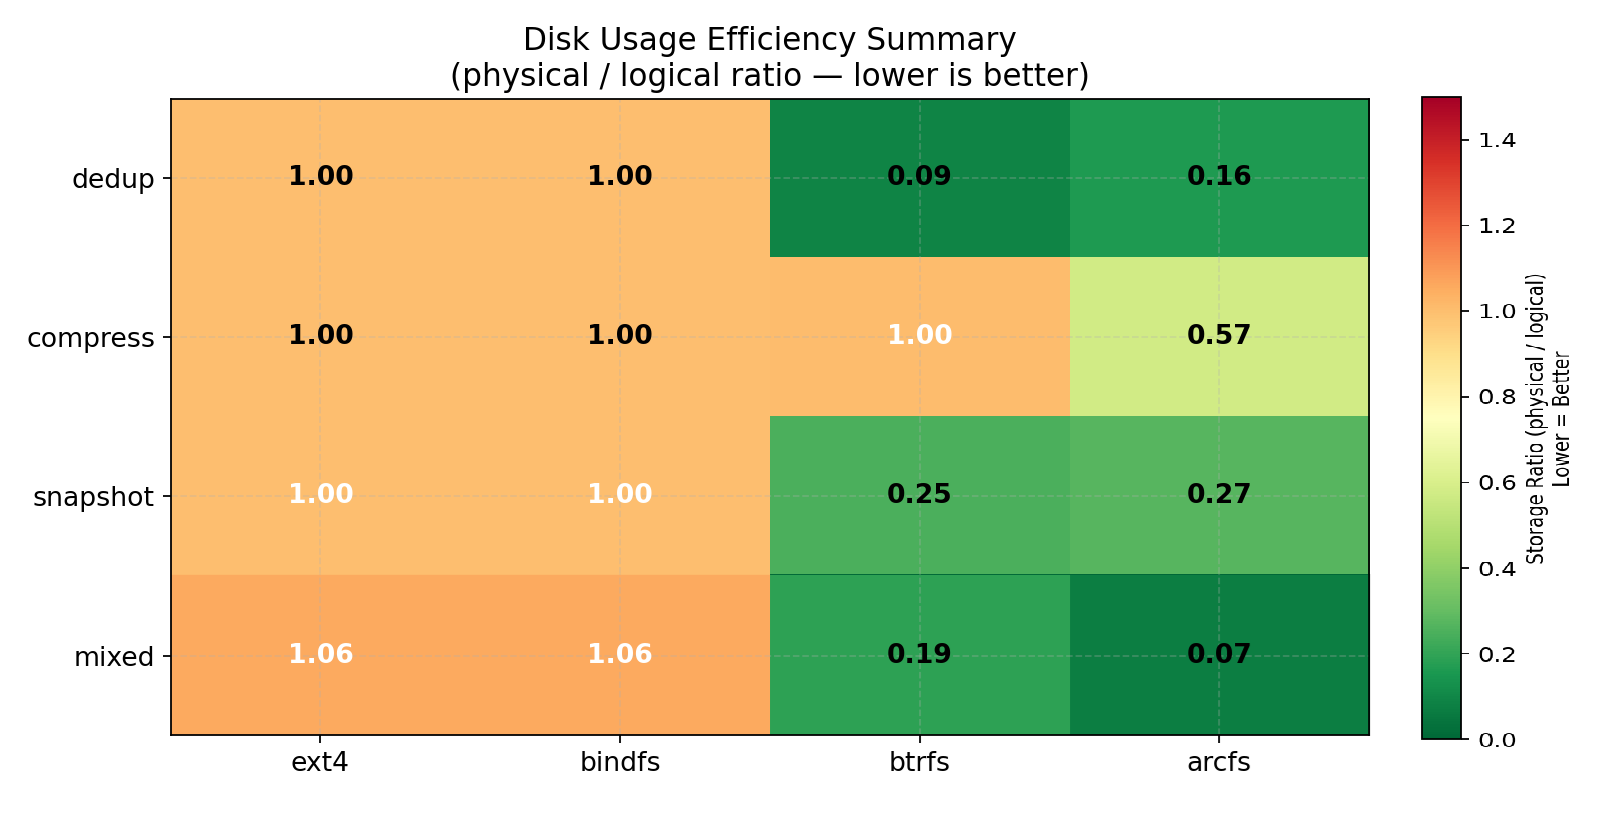
\includegraphics[width=\columnwidth]{figures/summary_heatmap.png}
\caption{Disk usage efficiency heatmap: physical-to-logical storage ratio
  (lower is better) across all four disk-usage profiles and all four
  filesystem targets. ArcFS achieves the lowest ratio on mixed (0.07)
  and compression (0.57 average) scenarios. Btrfs dominates on pure
  deduplication (0.016) via O(1) reflink but offers no compression
  benefit as mounted.}
\label{fig:heatmap}
\end{figure}

Figure~\ref{fig:heatmap} consolidates physical-to-logical storage ratios
across all profiles. Ext4 and bindfs form a uniform band at $\approx 1.0$.
Btrfs dominates on the deduplication profile (0.016 via reflink) and
performs well on snapshots (0.25), but offers no compression advantage as
mounted. ArcFS achieves the lowest ratio on mixed workloads (0.07) and
compression profiles (0.57 average) and closely matches Btrfs on snapshots
(0.27 vs. 0.25). Its weakest result is on pure deduplication (0.163
vs. Btrfs 0.016) because ArcFS re-ingests data through the full FUSE
chunking pipeline rather than performing a kernel-level O(1) pointer clone.

%% ─────────────────────────────────────────────────────────────────────────────
\section{Discussion}

\subsection{Two-Class Performance Trade-off}

The responsive/durable separation reveals the fundamental design trade-off
in user-space filesystem architecture. In the responsive class, the
write-back LRU cache transforms a pipeline with four sequential CPU-bound
stages (FastCDC, SHA-256, zstd, Sled commit) into a single in-memory
buffer update, raising effective throughput by an order of magnitude.
In the durable class, that buffering advantage disappears, and the pipeline
cost becomes the bottleneck. ArcFS remains competitive with kernel
filesystems in the durable class on most profiles, which confirms that the
four-stage pipeline does not introduce catastrophic overhead, only a
predictable latency proportional to per-write flush cost.

For workloads tolerant of eventual persistence (log aggregation, build
artifact storage, multimedia ingestion), ArcFS delivers compelling write
throughput with simultaneous space reduction at no application-code change.
For workloads demanding synchronous durability (database write-ahead logs,
transactional record systems), ArcFS provides correct behavior with
throughput near kernel baselines but not exceeding them.

\subsection{Overhead Sources and Limits}

Three overheads characterize ArcFS relative to kernel filesystems. First,
every FUSE request crosses the kernel/user boundary twice, adding latency
that accumulates on metadata-intensive workloads such as random 4\,KB
reads with cache misses. Second, the FastCDC pipeline introduces
measurable CPU work per flush: Gear-hash evaluation across the byte stream,
SHA-256 digest computation, zstd framing, and Sled transaction commit all
execute synchronously in the daemon. Third, pure incompressible data
incurs a 19\% storage overhead from CAS metadata structures, representing
the worst-case structural penalty for the pipelining design.

\subsection{Comparison with Prior Systems}

ArcFS occupies a design point approached only partially by prior work.
LBFS~\cite{muthitacharoen2001lbfs} performs CDC deduplication but at the
network layer, with no tag-based access or versioning. Btrfs provides
kernel-native CoW and snapshot efficiency but requires explicit mount
options (\texttt{compress=zstd}) and offline passes for compression and
cross-file deduplication, respectively. The Bento
system~\cite{miller2021bento} eliminates FUSE context-switch overhead
through Rust-based in-kernel modules but does not integrate deduplication
or semantic tagging. ArcFS combines CDC deduplication, CoW versioning,
and semantic tag navigation in a single POSIX-compatible user-space
prototype, achieving it without kernel modifications.

%% ─────────────────────────────────────────────────────────────────────────────
\section{Conclusion}

ArcFS demonstrates that a single Rust FUSE daemon can integrate
content-defined chunking, content-addressable storage, copy-on-write
versioning, and tag-based semantic navigation without sacrificing POSIX
compatibility or data correctness. In responsive workloads, the system
delivers $9.2\times$ sequential write throughput over ext4 by coalescing
I/O in a bounded-memory LRU cache. On storage efficiency, it achieves
83.7\% deduplication savings on identical files, reduces mixed-workload
disk consumption by 57.6\% over ext4, and holds snapshot storage costs
within 1.3$\times$ of kernel-native Btrfs. All CRC32c integrity
verifications pass at zero error rate, confirming lossless reconstruction
through the full chunking and decompression pipeline. Future work will
focus on crash recovery hardening through atomic metadata journaling,
parallel chunk processing to reduce durable-class flush latency,
and distributed CAS storage across multiple nodes to scale the system
beyond single-machine capacity.

%% ─────────────────────────────────────────────────────────────────────────────
\balance
\bibliographystyle{IEEEtran}
\bibliography{references}

\end{document}
